\documentclass{article}

\usepackage[letterpaper, margin=1in]{geometry}

\usepackage{titlesec}
%\usepackage[none]{hyphenat} % use only if there is a problem
% Use Unicode characters
\usepackage[utf8]{inputenc}

% tables
\usepackage{longtable,booktabs,array}
\usepackage{multirow}
\usepackage{afterpage}

% figures
\usepackage{wrapfig}
\usepackage{lscape}
\usepackage{rotating}
\usepackage{graphicx}
\graphicspath{assets}
\usepackage{times}
\usepackage{caption}

\title{Supplementary material for "Gut microbes and their genes are associated with cognition and neuroanatomy in children"}

\begin{document}

\baselineskip24pt

\maketitle

\begin{figure}[h]
    \centering
    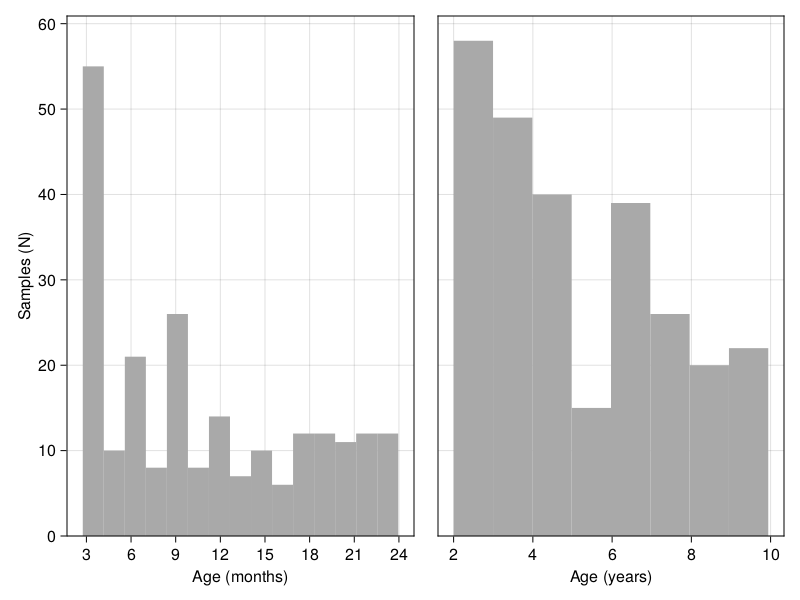
\includegraphics[width=0.9\textwidth]{assets/Supp_Figure1.png}
    \captionsetup{labelformat=empty}
    \caption{
        \textbf{Figure S1}: Sample collection by age - related to Figure 1A. A histogram showing the number of samples
        included in this study by the age of the child when the sample was collected.
    }
\end{figure}

\begin{figure}[h]
    \centering
    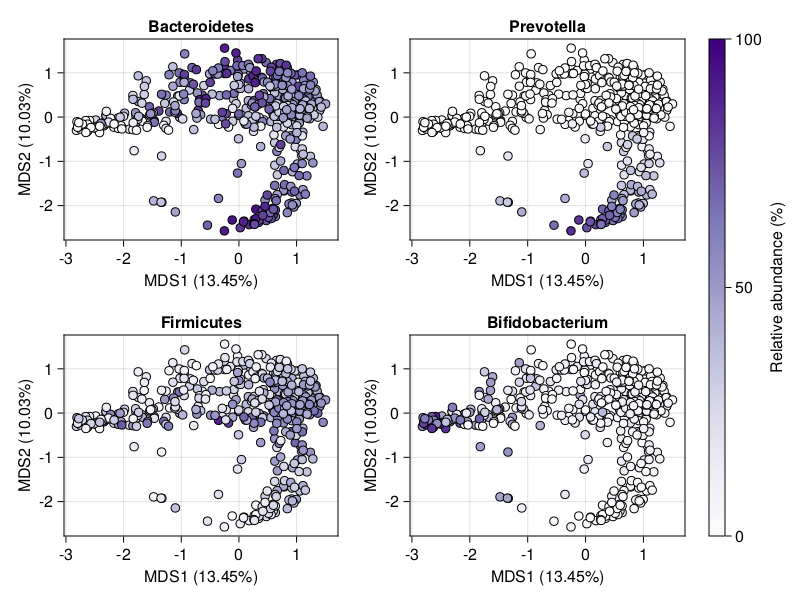
\includegraphics[width=0.9\textwidth]{assets/Supp_Figure2.png}
    \captionsetup{labelformat=empty}
    \caption{
        \textbf{Figure S2}: Principal coordinates analysis of taxonomic profiles - 
        related to Figure 1C. PCoAs are colored by the relative abundance per-sample
        of major phyla (Bacteroidetes, top left; Firmicutes, bottom left)
        and genera (\textit{Prevotella}, top right; \textit{Bifidobacterium}, bottom right).
    }
\end{figure}

\begin{figure}[h]
    \centering
    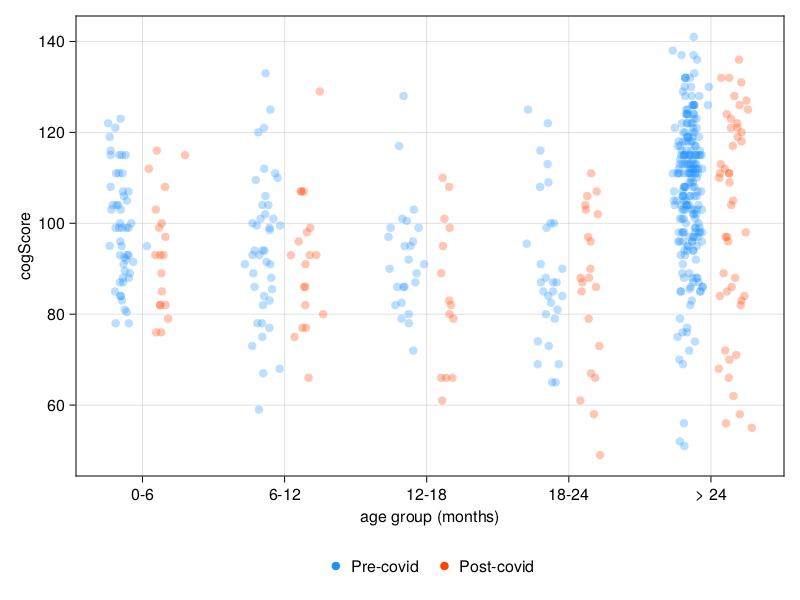
\includegraphics[width=0.9\textwidth]{assets/Supp_Figure3.png}
    \captionsetup{labelformat=empty}
    \caption{
        \textbf{Figure S3}: Cognitive assessment scores based on age
        and COVID-19. Scores in red were collected after March of 2020.
    }
\end{figure}

\begin{figure}[h]
  \centering
  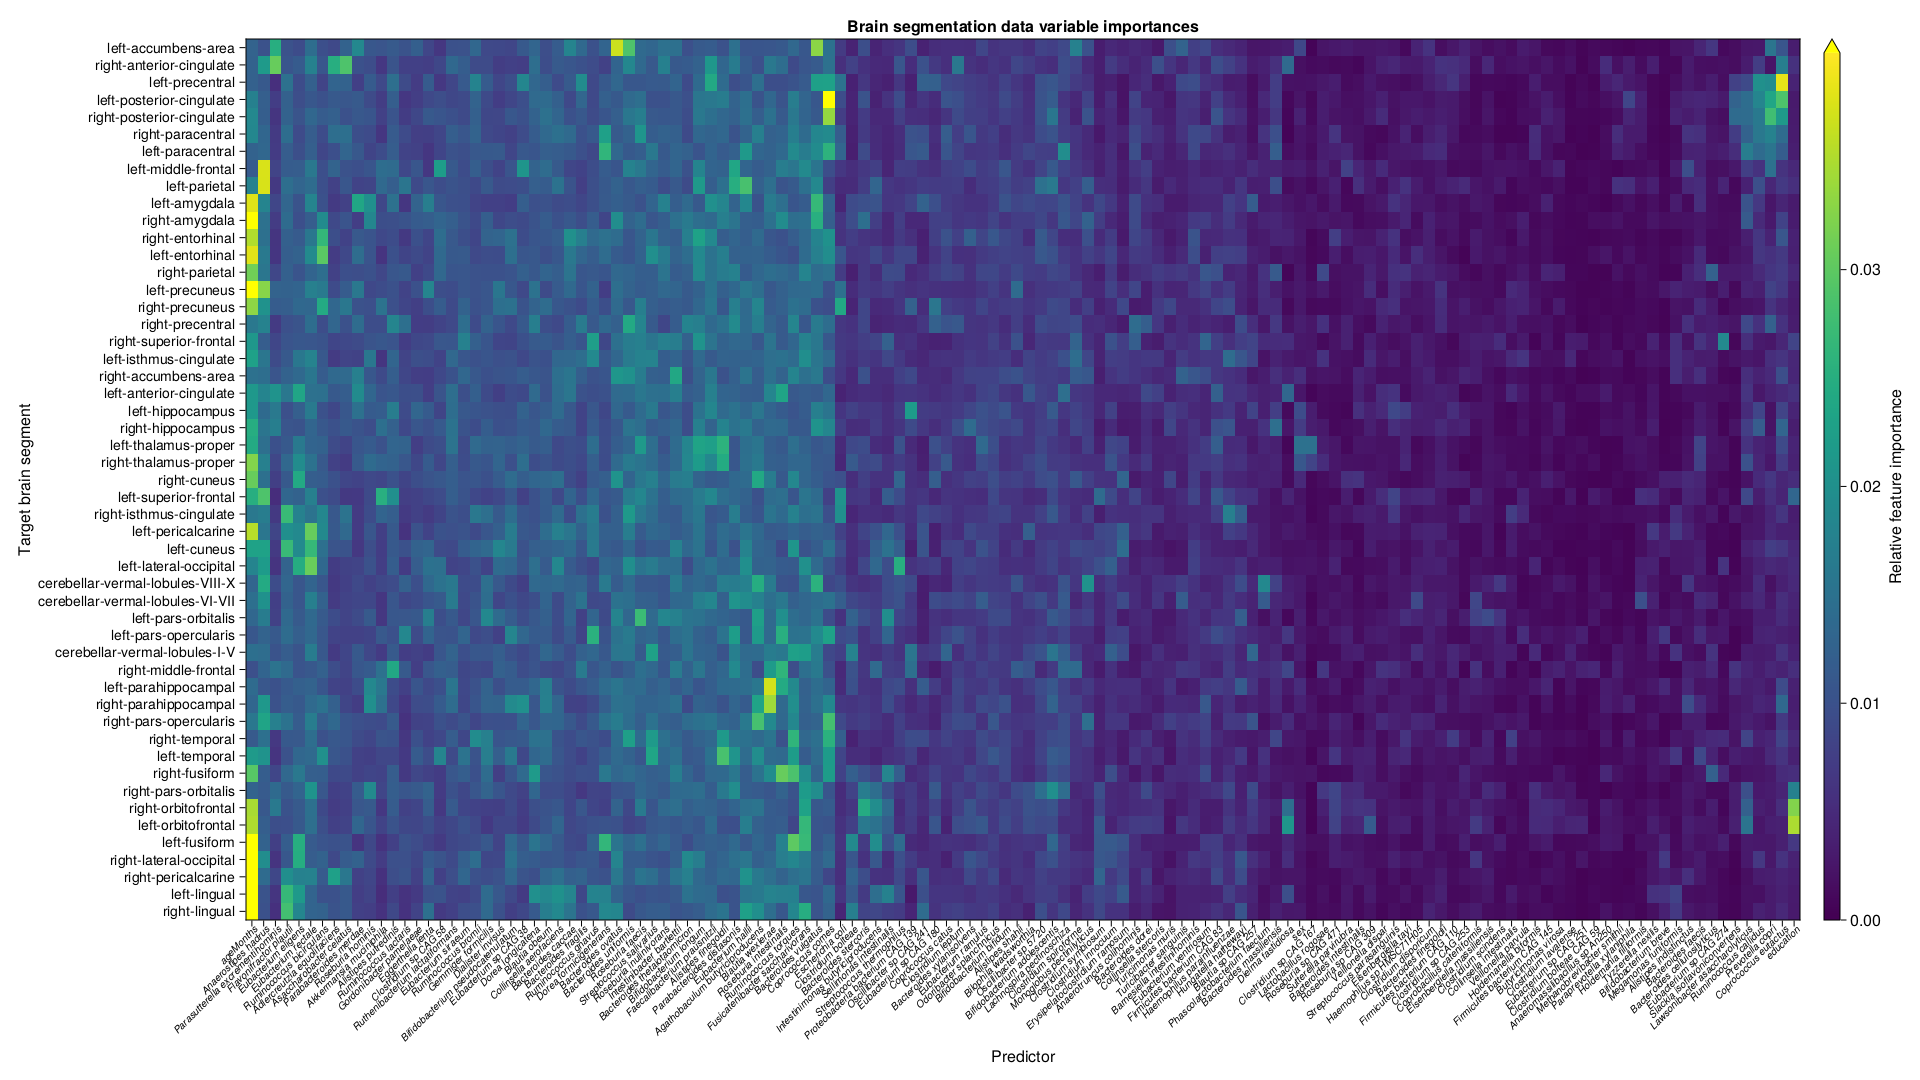
\includegraphics[width=0.9\textwidth]{assets/Supp_Figure5.png}
  \captionsetup{labelformat=empty}
  \caption{
      \textbf{Figure S5}: Species feature importances in brain region RFs - related to Figure 4C.
      All species (plus sex and maternal education) feature importances in each brain region model.
      X-axis is rank-ordered by median importance across all brain region models.
  }
\end{figure}

\begin{table}[h]
    \begin{centering}
    \tiny
    \begin{tabular}{|r|r|r|r|r|}
      \hline\hline
      \textbf{Rank} & \textbf{Variable} & \textbf{Average fitness-weighted importance} & \textbf{Relative fitness-weighted importance} & \textbf{Rank-cumulative relative importance } \\\hline
      1 & \textit{Erysipelatoclostridium ramosum} & 0.00455796 & 5.57 \% & 5.57 \% \\
      2 & \textit{ageMonths} & 0.00352354 & 4.31 \% & 9.88 \% \\
      3 & \textit{Eggerthella lenta} & 0.00312334 & 3.82 \% & 13.7 \% \\
      4 & \textit{Escherichia coli} & 0.00310493 & 3.8 \% & 17.5 \% \\
      5 & \textit{Bifidobacterium longum} & 0.00286972 & 3.51 \% & 21.01 \% \\
      6 & \textit{Veillonella parvula} & 0.00279249 & 3.42 \% & 24.43 \% \\
      7 & \textit{Bifidobacterium breve} & 0.00266183 & 3.26 \% & 27.68 \% \\
      8 & \textit{Klebsiella variicola} & 0.00243687 & 2.98 \% & 30.66 \% \\
      9 & \textit{Enterococcus faecalis} & 0.0023808 & 2.91 \% & 33.57 \% \\
      10 & \textit{Streptococcus salivarius} & 0.00232582 & 2.84 \% & 36.42 \% \\
      11 & \textit{Klebsiella pneumoniae} & 0.00230664 & 2.82 \% & 39.24 \% \\
      12 & \textit{Bifidobacterium bifidum} & 0.00211952 & 2.59 \% & 41.83 \% \\
      13 & \textit{Flavonifractor plautii} & 0.00208123 & 2.55 \% & 44.38 \% \\
      14 & \textit{Ruminococcus gnavus} & 0.00206215 & 2.52 \% & 46.9 \% \\
      15 & \textit{Veillonella atypica} & 0.00197072 & 2.41 \% & 49.31 \% \\
      16 & \textit{Klebsiella quasipneumoniae} & 0.00187371 & 2.29 \% & 51.6 \% \\
      17 & \textit{Gordonibacter pamelaeae} & 0.00177287 & 2.17 \% & 53.77 \% \\
      18 & \textit{Clostridioides difficile} & 0.00165027 & 2.02 \% & 55.79 \% \\
      19 & \textit{Clostridium innocuum} & 0.00152836 & 1.87 \% & 57.66 \% \\
      20 & \textit{Streptococcus parasanguinis} & 0.00141086 & 1.73 \% & 59.38 \% \\
      21 & \textit{Blautia wexlerae} & 0.0013505 & 1.65 \% & 61.03 \% \\
      22 & \textit{Bacteroides vulgatus} & 0.00134672 & 1.65 \% & 62.68 \% \\
      23 & \textit{Clostridium neonatale} & 0.00123595 & 1.51 \% & 64.19 \% \\
      24 & \textit{Enterococcus gallinarum} & 0.00114326 & 1.4 \% & 65.59 \% \\
      25 & \textit{Veillonella dispar} & 0.00108836 & 1.33 \% & 66.92 \% \\
      26 & \textit{Collinsella aerofaciens} & 0.00107748 & 1.32 \% & 68.24 \% \\
      27 & \textit{Clostridium paraputrificum} & 0.00104175 & 1.27 \% & 69.51 \% \\
      28 & \textit{Parabacteroides distasonis} & 0.00103126 & 1.26 \% & 70.78 \% \\
      29 & \textit{Collinsella stercoris} & 0.00102022 & 1.25 \% & 72.02 \% \\
      30 & \textit{Intestinibacter bartlettii} & 0.00100161 & 1.22 \% & 73.25 \% \\
      31 & \textit{Bacteroides uniformis} & 0.000992884 & 1.21 \% & 74.46 \% \\
      32 & \textit{Streptococcus mitis} & 0.00095161 & 1.16 \% & 75.63 \% \\
      33 & \textit{Bacteroides ovatus} & 0.000899836 & 1.1 \% & 76.73 \% \\
      34 & \textit{Klebsiella oxytoca} & 0.000897222 & 1.1 \% & 77.82 \% \\
      35 & \textit{Hungatella hathewayi} & 0.000843434 & 1.03 \% & 78.86 \% \\
      36 & \textit{Veillonella infantium} & 0.000801475 & 0.98 \% & 79.84 \% \\
      37 & \textit{Clostridium sp 7 2 43FAA} & 0.000774221 & 0.95 \% & 80.78 \% \\
      38 & \textit{Haemophilus parainfluenzae} & 0.000767324 & 0.94 \% & 81.72 \% \\
      39 & \textit{Parabacteroides merdae} & 0.000715631 & 0.88 \% & 82.6 \% \\
      40 & \textit{Clostridium bolteae} & 0.000680723 & 0.83 \% & 83.43 \% \\
      41 & \textit{Clostridium perfringens} & 0.000676374 & 0.83 \% & 84.26 \% \\
      42 & \textit{Bifidobacterium adolescentis} & 0.000666846 & 0.82 \% & 85.07 \% \\
      43 & \textit{Bifidobacterium pseudocatenulatum} & 0.000609418 & 0.75 \% & 85.82 \% \\
      44 & \textit{Enterococcus avium} & 0.000585969 & 0.72 \% & 86.53 \% \\
      45 & \textit{Bacteroides thetaiotaomicron} & 0.000571891 & 0.7 \% & 87.23 \% \\
      46 & \textit{Akkermansia muciniphila} & 0.000554837 & 0.68 \% & 87.91 \% \\
      47 & \textit{Bacteroides caccae} & 0.000545515 & 0.67 \% & 88.58 \% \\
      48 & \textit{Citrobacter youngae} & 0.000518293 & 0.63 \% & 89.21 \% \\
      49 & \textit{Sellimonas intestinalis} & 0.000510043 & 0.62 \% & 89.84 \% \\
      50 & \textit{Enterobacter cloacae complex} & 0.000493869 & 0.6 \% & 90.44 \% \\
      51 & \textit{Streptococcus thermophilus} & 0.000490258 & 0.6 \% & 91.04 \% \\
      52 & \textit{Lactobacillus rhamnosus} & 0.000474719 & 0.58 \% & 91.62 \% \\
      53 & \textit{Bacteroides stercoris} & 0.000456499 & 0.56 \% & 92.18 \% \\
      54 & \textit{Klebsiella michiganensis} & 0.000451312 & 0.55 \% & 92.73 \% \\
      55 & \textit{Enterococcus faecium} & 0.000363871 & 0.45 \% & 93.18 \% \\
      56 & \textit{Veillonella sp T11011 6} & 0.00035483 & 0.43 \% & 93.61 \% \\
      57 & \textit{Streptococcus vestibularis} & 0.000348252 & 0.43 \% & 94.04 \% \\
      58 & \textit{Ruthenibacterium lactatiformans} & 0.000340758 & 0.42 \% & 94.45 \% \\
      59 & \textit{Bacteroides fragilis} & 0.00033134 & 0.41 \% & 94.86 \% \\
      60 & \textit{Anaerostipes caccae} & 0.000323646 & 0.4 \% & 95.25 \% \\
      61 & \textit{Enterococcus casseliflavus} & 0.000321971 & 0.39 \% & 95.65 \% \\
      62 & \textit{Citrobacter freundii} & 0.000316149 & 0.39 \% & 96.03 \% \\
      63 & \textit{Proteus mirabilis} & 0.00031606 & 0.39 \% & 96.42 \% \\
      64 & \textit{Collinsella intestinalis} & 0.000306493 & 0.37 \% & 96.8 \% \\
      65 & \textit{Varibaculum cambriense} & 0.000300238 & 0.37 \% & 97.16 \% \\
      66 & \textit{Bilophila wadsworthia} & 0.000274898 & 0.34 \% & 97.5 \% \\
      67 & \textit{Bifidobacterium scardovii} & 0.000248479 & 0.3 \% & 97.8 \% \\
      68 & \textit{Aeriscardovia aeriphila} & 0.000238753 & 0.29 \% & 98.1 \% \\
      69 & \textit{Morganella morganii} & 0.000215584 & 0.26 \% & 98.36 \% \\
      70 & \textit{Bacteroides massiliensis} & 0.000207972 & 0.25 \% & 98.61 \% \\
      71 & \textit{Clostridium symbiosum} & 0.000181616 & 0.22 \% & 98.84 \% \\
      72 & \textit{Lactococcus lactis} & 0.000178531 & 0.22 \% & 99.05 \% \\
      73 & \textit{Bacteroides dorei} & 0.000165989 & 0.2 \% & 99.26 \% \\
      74 & \textit{Actinomyces sp HPA0247} & 0.000151331 & 0.19 \% & 99.44 \% \\
      75 & \textit{Bacteroides xylanisolvens} & 0.000110403 & 0.14 \% & 99.58 \% \\
      76 & \textit{Phascolarctobacterium faecium} & 9.67579e-5 & 0.12 \% & 99.7 \% \\
      77 & \textit{Streptococcus pasteurianus} & 8.79395e-5 & 0.11 \% & 99.8 \% \\
      78 & \textit{Fusicatenibacter saccharivorans} & 8.51867e-5 & 0.1 \% & 99.91 \% \\
      79 & \textit{Ruminococcus torques} & 7.57866e-5 & 0.09 \% & 100.0 \% \\\hline\hline
    \end{tabular}
    \caption*{
        \textbf{Table S1A}: Feature importances for RF models of cognitive performance
        based on taxonomic profiles in children under 6 months old.
    }
    \end{centering}
  \end{table}

\begin{table}[h]
  \begin{centering}
    \tiny
    \begin{tabular}{|r|r|r|r|r|}
      \hline\hline
      \textbf{Rank} & \textbf{Variable} & \textbf{Average fitness-weighted importance} & \textbf{Relative fitness-weighted importance} & \textbf{Rank-cumulative relative importance } \\\hline
      1 & \textit{ageMonths} & 0.0212894 & 6.48 \% & 6.48 \% \\
      2 & \textit{Faecalibacterium prausnitzii} & 0.00858801 & 2.61 \% & 9.09 \% \\
      3 & \textit{Bifidobacterium pseudocatenulatum} & 0.00597853 & 1.82 \% & 10.91 \% \\
      4 & \textit{Asaccharobacter celatus} & 0.00585523 & 1.78 \% & 12.7 \% \\
      5 & \textit{Eubacterium eligens} & 0.00536145 & 1.63 \% & 14.33 \% \\
      6 & \textit{Bifidobacterium longum} & 0.00535789 & 1.63 \% & 15.96 \% \\
      7 & \textit{Streptococcus parasanguinis} & 0.00517109 & 1.57 \% & 17.53 \% \\
      8 & \textit{Ruminococcus gnavus} & 0.00507375 & 1.54 \% & 19.08 \% \\
      9 & \textit{Roseburia faecis} & 0.00505688 & 1.54 \% & 20.62 \% \\
      10 & \textit{Bacteroides vulgatus} & 0.00481963 & 1.47 \% & 22.08 \% \\
      11 & \textit{Megamonas funiformis} & 0.00474784 & 1.45 \% & 23.53 \% \\
      12 & \textit{Fusicatenibacter saccharivorans} & 0.00470536 & 1.43 \% & 24.96 \% \\
      13 & \textit{Blautia wexlerae} & 0.00467839 & 1.42 \% & 26.38 \% \\
      14 & \textit{Roseburia hominis} & 0.00463749 & 1.41 \% & 27.79 \% \\
      15 & \textit{Eubacterium hallii} & 0.00462447 & 1.41 \% & 29.2 \% \\
      16 & \textit{Parasutterella excrementihominis} & 0.00439619 & 1.34 \% & 30.54 \% \\
      17 & \textit{Anaerostipes hadrus} & 0.00435503 & 1.33 \% & 31.87 \% \\
      18 & \textit{Blautia obeum} & 0.00412602 & 1.26 \% & 33.12 \% \\
      19 & \textit{Agathobaculum butyriciproducens} & 0.00394958 & 1.2 \% & 34.32 \% \\
      20 & \textit{Haemophilus parainfluenzae} & 0.00386417 & 1.18 \% & 35.5 \% \\
      21 & \textit{Gordonibacter pamelaeae} & 0.00380321 & 1.16 \% & 36.66 \% \\
      22 & \textit{Alistipes finegoldii} & 0.00375788 & 1.14 \% & 37.8 \% \\
      23 & \textit{Dorea longicatena} & 0.00373156 & 1.14 \% & 38.94 \% \\
      24 & \textit{Flavonifractor plautii} & 0.00364836 & 1.11 \% & 40.05 \% \\
      25 & \textit{Streptococcus salivarius} & 0.00361884 & 1.1 \% & 41.15 \% \\
      26 & \textit{Adlercreutzia equolifaciens} & 0.00355082 & 1.08 \% & 42.23 \% \\
      27 & \textit{Veillonella parvula} & 0.00354971 & 1.08 \% & 43.31 \% \\
      28 & \textit{Intestinibacter bartlettii} & 0.00349963 & 1.07 \% & 44.38 \% \\
      29 & \textit{Alistipes putredinis} & 0.00340834 & 1.04 \% & 45.41 \% \\
      30 & \textit{Ruthenibacterium lactatiformans} & 0.00335307 & 1.02 \% & 46.43 \% \\
      31 & \textit{Bacteroides ovatus} & 0.00330894 & 1.01 \% & 47.44 \% \\
      32 & \textit{Bacteroides fragilis} & 0.00330563 & 1.01 \% & 48.45 \% \\
      33 & \textit{Bacteroides uniformis} & 0.0033018 & 1.0 \% & 49.45 \% \\
      34 & \textit{Eubacterium rectale} & 0.00319986 & 0.97 \% & 50.43 \% \\
      35 & \textit{Roseburia inulinivorans} & 0.00307232 & 0.94 \% & 51.36 \% \\
      36 & \textit{Streptococcus thermophilus} & 0.00306275 & 0.93 \% & 52.29 \% \\
      37 & \textit{Roseburia intestinalis} & 0.00305426 & 0.93 \% & 53.22 \% \\
      38 & \textit{Bacteroides caccae} & 0.00298342 & 0.91 \% & 54.13 \% \\
      39 & \textit{Ruminococcus bicirculans} & 0.00295612 & 0.9 \% & 55.03 \% \\
      40 & \textit{Parabacteroides distasonis} & 0.00289418 & 0.88 \% & 55.91 \% \\
      41 & \textit{Ruminococcus torques} & 0.00286787 & 0.87 \% & 56.78 \% \\
      42 & \textit{Clostridium symbiosum} & 0.00283373 & 0.86 \% & 57.65 \% \\
      43 & \textit{Collinsella stercoris} & 0.00280616 & 0.85 \% & 58.5 \% \\
      44 & \textit{Bifidobacterium bifidum} & 0.00277992 & 0.85 \% & 59.35 \% \\
      45 & \textit{Collinsella aerofaciens} & 0.00277722 & 0.85 \% & 60.19 \% \\
      46 & \textit{Ruminococcus bromii} & 0.00275241 & 0.84 \% & 61.03 \% \\
      47 & \textit{Eubacterium sp CAG 38} & 0.00274717 & 0.84 \% & 61.87 \% \\
      48 & \textit{Erysipelatoclostridium ramosum} & 0.00269738 & 0.82 \% & 62.69 \% \\
      49 & \textit{Gemmiger formicilis} & 0.00265859 & 0.81 \% & 63.5 \% \\
      50 & \textit{Eggerthella lenta} & 0.00260529 & 0.79 \% & 64.29 \% \\
      51 & \textit{Dorea formicigenerans} & 0.00252851 & 0.77 \% & 65.06 \% \\
      52 & \textit{Parabacteroides merdae} & 0.00247422 & 0.75 \% & 65.81 \% \\
      53 & \textit{Odoribacter splanchnicus} & 0.00246359 & 0.75 \% & 66.56 \% \\
      54 & \textit{Bacteroides thetaiotaomicron} & 0.00245779 & 0.75 \% & 67.31 \% \\
      55 & \textit{Coprococcus eutactus} & 0.00245541 & 0.75 \% & 68.06 \% \\
      56 & \textit{Coprococcus comes} & 0.00244569 & 0.74 \% & 68.8 \% \\
      57 & \textit{Tyzzerella nexilis} & 0.00241174 & 0.73 \% & 69.54 \% \\
      58 & \textit{Megamonas hypermegale} & 0.00236407 & 0.72 \% & 70.25 \% \\
      59 & \textit{Ruminococcus lactaris} & 0.00236394 & 0.72 \% & 70.97 \% \\
      60 & \textit{Eubacterium siraeum} & 0.00234389 & 0.71 \% & 71.69 \% \\
      61 & \textit{Clostridium sp CAG 58} & 0.00226855 & 0.69 \% & 72.38 \% \\
      62 & \textit{Clostridium spiroforme} & 0.00225324 & 0.69 \% & 73.06 \% \\
      63 & \textit{Veillonella atypica} & 0.00218966 & 0.67 \% & 73.73 \% \\
      64 & \textit{Bifidobacterium adolescentis} & 0.0021441 & 0.65 \% & 74.38 \% \\
      65 & \textit{Monoglobus pectinilyticus} & 0.00211824 & 0.64 \% & 75.03 \% \\
      66 & \textit{Alistipes shahii} & 0.00210389 & 0.64 \% & 75.67 \% \\
      67 & \textit{Eubacterium ramulus} & 0.00210011 & 0.64 \% & 76.31 \% \\
      68 & \textit{Prevotella copri} & 0.00208789 & 0.64 \% & 76.94 \% \\
      69 & \textit{Bacteroides xylanisolvens} & 0.00202167 & 0.62 \% & 77.56 \% \\
      70 & \textit{Oscillibacter sp 57 20} & 0.00201112 & 0.61 \% & 78.17 \% \\
      71 & \textit{Blautia sp CAG 257} & 0.00198307 & 0.6 \% & 78.77 \% \\
      72 & \textit{Sutterella parvirubra} & 0.0019804 & 0.6 \% & 79.38 \% \\
      73 & \textit{Akkermansia muciniphila} & 0.00192189 & 0.58 \% & 79.96 \% \\
      74 & \textit{Clostridium bolteae} & 0.00186087 & 0.57 \% & 80.53 \% \\
      75 & \textit{Clostridium leptum} & 0.00185445 & 0.56 \% & 81.09 \% \\
      76 & \textit{Lachnospira pectinoschiza} & 0.00184894 & 0.56 \% & 81.66 \% \\
      77 & \textit{Bacteroides stercoris} & 0.00184674 & 0.56 \% & 82.22 \% \\
      78 & \textit{Clostridium innocuum} & 0.00183522 & 0.56 \% & 82.78 \% \\
      79 & \textit{Escherichia coli} & 0.00182675 & 0.56 \% & 83.33 \% \\
      80 & \textit{Eubacterium sp CAG 180} & 0.00179463 & 0.55 \% & 83.88 \% \\
      81 & \textit{Intestinimonas butyriciproducens} & 0.00179373 & 0.55 \% & 84.42 \% \\
      82 & \textit{Dialister invisus} & 0.00176827 & 0.54 \% & 84.96 \% \\
      83 & \textit{Anaerotruncus colihominis} & 0.00170721 & 0.52 \% & 85.48 \% \\
      84 & \textit{Bifidobacterium breve} & 0.00167934 & 0.51 \% & 85.99 \% \\
      85 & \textit{Sellimonas intestinalis} & 0.0016637 & 0.51 \% & 86.5 \% \\
      86 & \textit{Veillonella infantium} & 0.00162428 & 0.49 \% & 86.99 \% \\
      87 & \textit{Bacteroides dorei} & 0.00160753 & 0.49 \% & 87.48 \% \\
      88 & \textit{Proteobacteria bacterium CAG 139} & 0.00160147 & 0.49 \% & 87.97 \% \\
      89 & \textit{Megamonas funiformis CAG 377} & 0.00151627 & 0.46 \% & 88.43 \% \\
      90 & \textit{Bilophila wadsworthia} & 0.00151572 & 0.46 \% & 88.89 \% \\
      91 & \textit{Hungatella hathewayi} & 0.00144508 & 0.44 \% & 89.33 \% \\
      92 & \textit{Veillonella dispar} & 0.0014432 & 0.44 \% & 89.77 \% \\
      93 & \textit{Turicimonas muris} & 0.00141116 & 0.43 \% & 90.2 \% \\
      94 & \textit{Roseburia sp CAG 471} & 0.00140979 & 0.43 \% & 90.63 \% \\
      95 & \textit{Eisenbergiella massiliensis} & 0.00137139 & 0.42 \% & 91.05 \% \\
      96 & \textit{Firmicutes bacterium CAG 83} & 0.00127233 & 0.39 \% & 91.44 \% \\
      97 & \textit{Barnesiella intestinihominis} & 0.00126284 & 0.38 \% & 91.82 \% \\
      98 & \textit{Turicibacter sanguinis} & 0.00122404 & 0.37 \% & 92.19 \% \\
      99 & \textit{Bifidobacterium catenulatum} & 0.00117205 & 0.36 \% & 92.55 \% \\
      100 & \textit{Bacteroides finegoldii} & 0.00114999 & 0.35 \% & 92.9 \% \\
      100+ & See Table file & ... & ... & ... \\\hline\hline

    \end{tabular}
    \caption*{
        \textbf{Table S1B}: Feature importances for RF models of cognitive performance
        based on taxonomic profiles in children over 18 months old.
    }
    \end{centering}
  \end{table}

  \begin{table}[h]
  
  \begin{centering}
    \tiny
    \begin{tabular}{|r|r|r|}
      \hline\hline
      \textbf{Segment} & \textbf{Mean absolute proportional error (MAPE)} & \textbf{Correlation coefficient (R)} \\\hline
      Left temporal & 0.0404594 & 0.127818 \\
      Right temporal & 0.0392704 & 0.0682501 \\
      Left orbitofrontal & 0.055416 & 0.186246 \\
      Right orbitofrontal & 0.0614151 & 0.132539 \\
      Left parietal & 0.0351769 & 0.17665 \\
      Right parietal & 0.0451491 & -0.147144 \\
      Left middle frontal & 0.0520623 & -0.000244763 \\
      Right middle frontal & 0.0385468 & 0.0828596 \\
      Left anterior cingulate & 0.0685289 & 0.0917192 \\
      Right anterior cingulate & 0.0739281 & 0.244738 \\
      Left lateral occipital & 0.0621555 & 0.223683 \\
      Right lateral occipital & 0.0543598 & 0.220757 \\
      Left cerebellum white matter & 0.066747 & 0.413219 \\
      Right cerebellum white matter & 0.0697708 & 0.434406 \\
      Left thalamus proper & 0.0533751 & 0.169561 \\
      Right thalamus proper & 0.049911 & 0.161614 \\
      Left caudate & 0.098966 & 0.0287327 \\
      Right caudate & 0.0829818 & -0.0100022 \\
      Left putamen & 0.0592467 & 0.154136 \\
      Right putamen & 0.0658062 & 0.0106574 \\
      Left pallidum & 0.0640696 & 0.296669 \\
      Right pallidum & 0.061284 & 0.264402 \\
      Left hippocampus & 0.0541142 & 0.0749129 \\
      Right hippocampus & 0.0592959 & -0.0936672 \\
      Left amygdala & 0.0631678 & 0.287858 \\
      Right amygdala & 0.0704248 & 0.178656 \\
      Left accumbens area & 0.0940644 & 0.287736 \\
      Right accumbens area & 0.102421 & -0.0406411 \\
      Left basal forebrain & 0.205866 & 0.15437 \\
      Right basal forebrain & 0.116891 & 0.123397 \\
      Left cuneus & 0.0815679 & 0.23447 \\
      Right cuneus & 0.0749546 & 0.0646581 \\
      Left entorhinal & 0.0798131 & 0.190416 \\
      Right entorhinal & 0.0822284 & 0.0992957 \\
      Left fusiform & 0.0572084 & 0.333085 \\
      Right fusiform & 0.0530445 & 0.248232 \\
      Left isthmus cingulate & 0.0773557 & -0.0409419 \\
      Right isthmus cingulate & 0.0853975 & 0.0735448 \\
      Left lingual & 0.0688078 & 0.421223 \\
      Right lingual & 0.0718747 & 0.433618 \\
      Left parahippocampal & 0.0575556 & 0.153532 \\
      Right parahippocampal & 0.0601658 & 0.134136 \\
      Left paracentral & 0.0781315 & 0.130863 \\
      Right paracentral & 0.0840377 & 0.0231437 \\
      Left pars opercularis & 0.0570367 & 0.14639 \\
      Right pars opercularis & 0.0595218 & 0.0301463 \\
      Left pars orbitalis & 0.0820972 & 0.00319405 \\
      Right pars orbitalis & 0.11185 & 0.0235441 \\
      Left pars triangularis & 0.063322 & 0.174337 \\
      Right pars triangularis & 0.0761507 & 0.0433894 \\
      Left pericalcarine & 0.110546 & 0.199714 \\
      Right pericalcarine & 0.0885021 & 0.272855 \\
      Left postcentral & 0.0515561 & 0.168095 \\
      Right postcentral & 0.0594766 & 0.134867 \\
      Left posterior cingulate & 0.133826 & 0.136535 \\
      Right posterior cingulate & 0.139374 & 0.0627632 \\
      Left precentral & 0.0653943 & 0.247774 \\
      Right precentral & 0.0463051 & 0.0656041 \\
      Left precuneus & 0.0561127 & 0.144285 \\
      Right precuneus & 0.0684661 & 0.149934 \\
      Left superior frontal & 0.0398019 & 0.100811 \\
      Right superior frontal & 0.0435653 & -0.0961327 \\
      Left supramarginal & 0.0667543 & 0.0611083 \\
      Right supramarginal & 0.0681908 & -0.000755991 \\
      Left insula & 0.0570695 & -0.118953 \\
      Right insula & 0.0561507 & 0.0770771 \\
      Cerebellar vermal lobules I V & 0.0846435 & 0.156162 \\
      Cerebellar vermal lobules VI VII & 0.0812733 & 0.00596907 \\
      Cerebellar vermal lobules VIII X & 0.0825333 & 0.0781431 \\
      Brain stem & 0.0765924 & 0.604747 \\
      CSF & 0.162364 & 0.0712952 \\\hline\hline
    \end{tabular}
    \caption*{
        \textbf{Table S2}: RF model performances predicting cortical and
        subcortical brain regions.
    }
    \end{centering}
  \end{table}


\begin{table}[h]
  \begin{centering}
    \begin{tabular}{|r|r|r|r|}
      \hline\hline
      \textbf{Input set} & \textbf{Age bracket} & \textbf{Microbiome encoding type} & \textbf{Demographics Provided? (sex, education)} \\\hline
      1 & \multirow{5}{*}{0 to 6 months} & Not provided & yes \\ \cline{3-4}
      2 &  & \multirow{2}{*}{Taxonomic profile} & no \\ \cline{4-4}
      3 &  &  & yes \\ \cline{3-4}
      4 &  & \multirow{2}{*}{Functional Profile (ECs)} & no \\ \cline{4-4}
      5 &  &  & yes \\ \cline{2-4}
      6 & \multirow{5}{*}{18 to 120 months} & Not provided & yes \\ \cline{3-4}
      7 &  & \multirow{2}{*}{Taxonomic profile} & no \\ \cline{4-4}
      8 &  &  & yes \\ \cline{3-4}
      9 &  & \multirow{2}{*}{Functional Profile (ECs)} & no \\ \cline{4-4}
      10 &  &  & yes \\\hline\hline
    \end{tabular}
    \caption*{
      \textbf{Table S3}: Experimental design and input composition for Random
      Forest experiments.
    }
  \end{centering}
\end{table}

\end{document}